
\problem{22.2-6}

There are two types of professional wrestlers: ``good guys'' and ``bad guys''. Between any pair of professional wrestlers, there may or may not be a rivalry. Suppose we have $n$
professional wrestlers and we have a list of $r$ pairs of wrestlers for which there are rivalries. Give an $O(n + r)$-time algorithm that determines whether it is possible to designate
some of the wrestlers as good guys and the remainder as bad guys such that each rivalry is between a good guy and a bad guy. If it is possible to perform such a designation, your
algorithm should produce it.
\answer
We can create a graph for the problem by making vertices for wrestlers, and edges for rivalry pairs, then paint it with 2 ``colors'': ``good'' or ``bad''.
The designation is possible only when there is a painting of the graph that no edge has same color on its two ends.

The algorithm works like this. Create a graph $G=(V, E)$ for the problem: each vertex represents a wrestler, and each edge represents a rivalry pair.
Visit the graph in a DFS fashion, and paints the vertices. Make sure that in the DFS tree, child vertices and parent vertex has different color.
Then check if for each edge, the two ends has different color.

Now we analysis the running time. Creating the graph takes $O(n + r)$ time; visiting and coloring takes $O(n + r)$ time; and finally checking the edges takes $O(r)$ time. So the
overall running time is in $O(n + r)$.
\qed

\problem{22.3-12}
A directed graph $G=(V, E)$ is \textsl{\textbf{singly connected}} if $u \leadsto v$ implies that there is at most one simple path from $u$ to $v$ for all vertices $u, v \in V$.
Give an efficient algorithm to determine whether or not a directed graph is singly connected.
\answer
% got this from pdfqueen
For each vertex $v\in V$, perform a DFS on $G$. Check if there is any forward edges or cross edges in the same component in any one of the DFS trees. If no such edges exists, then the
graph is \textbf{\textsl{singly connected}}, otherwise it is not. The overall complexity is $O(V(V+E))$.
\qed

\problem{22.4-2}
Give a linear-time algorithm that takes as input a directed acyclic graph $G=(V, E)$ and two vertices $s$ and $t$, and returns the number of paths from $s$ to $t$ in $G$. For example,
in the directed acyclic graph of the following graph, there are exactly four paths from vertex $p$ to vertex $v$: $pov, poryv, posryv$, and $psryv$. (Your algorithm only needs to count the
paths, not list them.)
\begin{center}
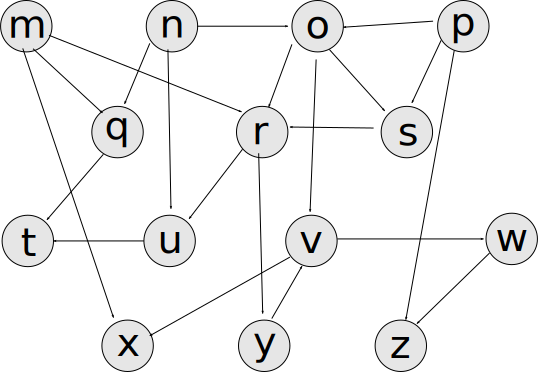
\includegraphics[width=120pt]{hw5-fig-22-8.pdf}
\end{center}
\answer
Denote the number of paths from $s$ to $u$ by $P(s, u)$, we calculate it recursively by
\begin{equation*}
P(s, u)=\left\{\begin{array}{ll}
\sum_{w \leadsto u}P(s, w)& (u \neq s)\\
0 & (u = s)\\
\end{array}\right.
\end{equation*}
Note that if a vertex $u$ does not have a parent, then $\sum_{w\leadsto u}P(s, w) = 0$, since there are no such parent $w$ vertices. And since the input is directed acyclic
graph, the recursion will terminate.

The algorithm is given below, an array $P$ is used to cache caculated results. $P$ is empty when calling for the first time.

\begin{algorithm}[H]
\caption{\textsc{Path-Count}$(G, P, s, t)$}
\If{$s = t$}{
  \Return $1$\\
}\Else{
  $S \leftarrow 0$\\
  \ForEach{parent vertex $w$ of $t$}{
    \If{$P[w]$ = nil} {
      $P[w]\leftarrow $\textsc{Path-Count}$(G, P, s, w)$
    }
    $S\leftarrow S + P(w)$
  }
  \Return $S$
}
\end{algorithm}

Line $4 \& 7$ is executed $O(V)$ times; line $6\&8$ is executed $O(E)$ times, since every edge will be checked only once when finding parent vertices. Thus we know the overall running time will be $O(V + E)$.
\qed

\problem{22.5-7}
A directed graph $G=(V, E)$ is said to be \textbf{\textsl{semiconnected}} if, for all pairs of vertices $u, v\in V$, we have $u\leadsto v$ or $v\leadsto u$. Give an efficient algorithm
to determine whether or not $G$ is semiconnected. Prove that your algorithm is correct, and analyze its running time.

\answer
First of all, we give the algorithm:

\begin{algorithm}[H]
\caption{\textsc{Is-Semiconnected}$(G)$}
$G' \leftarrow $\textsc{Strongly-Connected-Components}$(G)$\\
\If {$|V(G')|=1$}{
  \Return True
}\Else {
  $L \leftarrow$\textsc{Topological-Sort}$(G')$\\
  \For{$i = 1$ to $length[L]-1$}{
    \If{$(L[i], L[i + 1]) \notin E(G')$}{
      \Return False
    }
  }
  \Return True
}
\end{algorithm}

Now we explain how it works. It is trivial that strongly connected components are \textbf{\textsl{semiconnected}}, so first we shrink the original graph $G$ into $G'$ by finding
its strongly connected components. If $G'$ has only one vertex, it means the whole graph $G$ is strongly connected and thus \textbf{\textsl{semiconnected}}.
Otherwise, we run \textsc{Topological-Sort} on graph $G'$, line up its nodes in a list $L$. And then we check if any consecutive pair of vertices in $L$ is connected by an edge in $G'$.
If it is true, then for any $s, t\in G$, we can find corresponding $s', t'\in G'$ (and suppose $s'\neq t'$, in which case they are in the same strongly connected
components, and is discussed above), and either $s' \rightarrow L[i]\rightarrow L[i + 1] \rightarrow \cdots \rightarrow t'$
or $t' \rightarrow L[j] \rightarrow L[j + 1] \rightarrow \cdots \rightarrow s'$ in $L$. Thus we claim the graph $G$ is \textbf{\textsl{semiconnected}}.

Now we prove the algorithm is correct. According to the explanation above, \textsc{Is-Semiconnected} returns true only when the graph is \textbf{\textsl{semiconnected}}.
Suppose \textsc{Is-Semiconnected} returns false, which only happens when there is $(L[k], L[k + 1])\notin E(G')$. Since $L$ is a topological sort of $G'$, it is impossible
that $L[k + 1] \leadsto L[k]$. Now we have proved that neither $L[k] \leadsto L[k + 1]$ nor $L[k + 1] \leadsto L[k]$. So by choosing $s, v\in G$ corresponding to $L[k], L[k +1]\in G'$,
the graph $G$ cannot be \textbf{\textsl{semiconnected}}. Thus \textsc{Is-Semiconnected} returns false only when the graph is not \textbf{\textsl{semiconnected}}.

Finally, since both \textsc{Strongly-Connected-Components} \& \textsc{Topological-Sort} could be done in $O(V + E)$, and line $7$ is executed $O(V)$ times (at most $V$ items in $L$),
we know that \textsc{Is-Semiconnected} runs in $O(V + E)$.
\qed


\problem{22-2 Articulation points, bridges, and biconnected components}
Let $G=(V, E)$ be a connected, undirected graph. An \textbf{\textsl{articulation point}} of $G$ is a vertex whose removal disconnects $G$. A \textbf{\textsl{bridge}} of $G$ is an edge
whose removal disconnects $G$. A \textbf{\textsl{biconnected component}} of $G$ is a maximal set of edges such that any two edges in the set lie on a common simple cycle. The following figure
illustrates these definitions. We can determine articulation points, bridges, and biconnected components using depth-first search. Let $G_{\pi} = (V, E_\pi)$ be a depth-first tree of
$G$.

\begin{center}
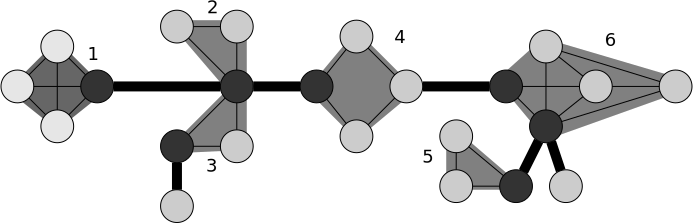
\includegraphics[width=300pt]{hw5-fig-22-10.pdf}
\end{center}

{
\small{
The articulation points, bridges and biconnected components of a connected, undirected graph for use in this problem. The articulation points are the heavily shaded vertices, teh bridges
are the heavily shaded edges, and the biconnected components are the edges in the shaded regions, with a $bcc$ number shown.}
}

\begin{description}
\item[a. \hspace{9pt}] Prove that the root of $G_\pi$ is an articulation point of $G$ if and only if it has at least two children in $G_\pi$.

\item[b. \hspace{9pt}] Let $v$ be a nonroot vertex of $G_\pi$. Prove that $v$ is an articulation point of $G$ if and only if $v$ has a child $s$ such that there is no back edge from $s$ or
any descendant of $s$ to a proper ancestor of $v$.

\item[c. \hspace{9pt}] Let
\begin{equation*}
low[v] = \min\left\{
  \begin{array}{l}
    d[v],\\
    d[w]:(u, w)\text{is a back edge for some descendent $u$ of $v$.}
  \end{array}
\right.
\end{equation*}

Show how to compute $low[v]$ for all vertices $v\in V$ in $O(E)$ time.

\item[d. \hspace{9pt}] Show how to compute all articulation points in $O(E)$ time.

\item[e. \hspace{9pt}] Prove that an edge of $G$ is a bridge if and only if it does not lie on any simple cycle of $G$.

\item[f. \hspace{9pt}] Show how to comput all the bridges of $G$ in $O(E)$ time.

\item[g. \hspace{9pt}] Prove that the biconnected components of $G$ partition the nonbridge edges of $G$.

\item[h. \hspace{9pt}] Give an $O(E)$-time algorithm to label each edge $e$ of $G$ with a positive integer $bcc[e]$ such that $bcc[e] = bcc[e']$ if and only if $e$ and $e'$ are
in the same biconnected component.

\end{description}
\answer

\begin{description}

\item[a. \hspace{9pt}] 

\textbf{root of $G_\pi$ is articulation point $\Rightarrow$ it has at least two children in $G_\pi$ :}

We prove by contradiction. Label the root point as $V_{root}$, and suppose it has less than 2 children in $G_\pi$. If $V_{root}$ has no children, then $V_{root}$ is the only
vertex in $G_pi$, and it is trivial that $V_{root}$ cannot be an articulation point. If $V_{root}$ has only one children $V_1$, then cutting $V_{root}$ off in  $G$ will still
left the subtree with root at $V_1$ connected, thus $V_{root}$ cannot be an articulation point. So $V_{root}$ must has at least 2 children in $G_\pi$. \\

\textbf{root of $G_\pi$ has at least two children in $G_\pi$ $\Rightarrow$ it is articulation point :}

Choose 2 children of $V_{root}$, label them as $V_1, V_2$, and the corresponding subtrees as $T_1, T_2$. First of all, there cannot be vertices $u\in T_1, v\in T_2$ such that $(u, v)\in E$,
otherwise according to DFS algorithm, $u, v$ should be in the same subtree, which is a contradiction to the fact that  $T_1 \cap T_2=\emptyset$. So by cutting $V_{root}$ off, subtree $T_1$ and $T_2$
will be disconnected, which means $V_{root}$ is an articulation point.

\item[b. \hspace{9pt}]

\textbf{``if'' side :}
% got this from pdfqueen
Assume that $v$ is an articulation point of $G$. Let $C_r$ be the connected component of $G-v$ containing the root of the tree $G_{\pi}$. Let $s$ be a neighbor of $v$ that is not in $C_r$
(this neighbor must exist since removing $v$ must create at least two connected components) and $C_s$ be the connected component containing $s$. In $G_\pi$, all the proper ancestors of
$v$ are in $C_r$, and all the descendants of $s$ are in $C_s$. Thus, there can be no edges between descendants of $s$ and proper ancestors of $v$.

\textbf{``only if'' side :}

Label the subtree at $v$ as $T_v$, and subtree at $s$ as $T_s$. By DFS algorithm, it is trivial that no vertex in $T_s$ could be connected to its sibling subtrees, so is true with $T_v$.
So we know that no vertex in $T_s$ could be connected to sibling trees of $T_s$, or $T_v$. And since no vertex in $T_s$ is connected to a proper ancestor of $v$, we know that by cutting
$v$ off, the whole subtree $T_s$ is disconected from other part of the graph. So $v$ is an articulation point.

\item[c. \hspace{9pt}]
% got this from pdfqueen
 
We can compute $low[v]$ for all vertices $v$ by starting at the leaves of the tree $G_\pi$. We compute $low[v]$ as follows:

$$low[v] = \min\left(d[v], \min_{y\in children(v)}low[y], \min_{backedge(v, w)}d[w]\right).$$

For leaves $v$, there are no descendants $u$ of $v$, so this returns either $d[v]$ or $d[w]$ if there is a back edge $(v, w)$. For vertices $v$ in the tree, if $low[v] = d[w]$, then either
there is a back edge $(v, w)$, or there is a back edge for some descendant $u$. The last term in the $\min$ expression handles the case where $(v, w)$ is a back edge. If $u$ is a descendant of
$v$ in $G_\pi$, we know that $d[u] > d[v]$ since $u$ is visited after $v$ in the DFS. Therefore, if $d[w] < d[v]$, we also have $d[w]< d[u]$, so we will have $low[u] = d[w]$. The middle term
in the $\min$ expression therefore handles the cases where $(u, w)$ is a back edge for some descendant $u$. Since we start at the leaves of the tree and work our way up, we will have computed
everything we need when computing $low[v]$.

For each node $v$, we look at $d[v]$ and something related to all the edges leading from $v$, either tree edges leading to the children or back edges. So, the total running time is linear in
the number of edges in $G$, i.e., $O(E)$.

\item[d. \hspace{9pt}] From (c) we could infer that $low[v] \leq d[v] \iff v$ is an articulation point. So we could find all the articulation points while calculating $low$ values.
Since calculation of $low$ value takes $O(E)$ time, finding articulation points will also take $O(E)$ time.

\item[e. \hspace{9pt}]

\textbf{``if'' side :}

Label the edge as $e^* = (u, v)$. We prove by contradiction. Suppose $e^*$ lies on a simple cycle $u - v - w_1 - w_2 - \cdots w_k - u$ of $G$. Consider 2 vertices $x, y$ which
is connected by path $x-x_1 -\cdots x_i - u - v - y_1 - y_2 \cdots y_j - y$. When $e^*$ is removed, $x, y$ is still connected by path $x - x_1 - \cdots x_i - u - w_k - \cdots w_1 -v- y_1 -
\cdots y_j -y$. Thus removing $e^*$ will not change the connectivity of $G$, which is a contradiction. From this we have proved  the ``if'' side.

\textbf{``only if'' side :}
% got this from pdfqueen

We prove by contradiction. Assume $(u, v)$ is not on a simple cycle, and it is not a bridge. Now remove the edge $(u, v)$. Since $(u, v)$ is not a bridge, there is still another path
connecting $u$ and $v$, say $u -x_1 -\cdots -x_i - v$. Then, the edges $u - v - x_i -\cdots-x_1 - u$ is a cycle, which is a contradiction. So $(u, v)$ must be a bridge.

\item[f. \hspace{9pt}] 
% got this from pdfqueen

Any bridge in the graph $G$ must exist in the graph $G_\pi$. Otherwise, assume $(u, v)$ is a bridge and that we explore $u$ first. Since removing $(u, v)$ disconnects $G$, the only way to
explore $v$ is through the edge $(u, v)$. So, we only need to consider the edges in $G_\pi$ as bridges. If there are no simple cycles in the graph that contains the edge $(u, v)$ and we
explore $u$ first, then we know that there are no back edges between $v$ and anything else. Also, we know that anything in the subtree of $v$ can only have back edges to other nodes in 
the subtree of $v$. Therefore, we will have $low[v] = d[v]$ since $v$ is the first node visited in the subtree rooted at $v$. Thus, we can look over all the edges of $G_\pi$ and see
whether $low[v] = d[v]$. If so, then we will output that $(parent[v]_{g_\pi}, v)$ is a bridge, i.e. that $v$ and its parent in $G_\pi$ form a bridge. Computing $low[v]$ for all vertices
$v$ takes time $O(E)$ as we showed in (c). Looping over all the edges takes time $O(V)$ since there are $(V-1)$ edges in $G_\pi$. Thus the total time to calculate the bridges in $G$ is
$O(E)$.

\item[g. \hspace{9pt}]
% got this from pdfqueen

Since \textbf{an edge is a bridge of $G \iff$  it is not on any simple cycle of $G$}, it is equivalent to the fact that \textbf{an edge is a nonbridge edge $\iff$ it is on any simple cycle of $G$}. Since
\textbf{an edge is in the biconnected component $\iff$ it is on any simple cycle of $G$}, we get the fact that \textbf{if the edge is in the biconnected components of $G \iff $ it is a nonbridge edge}.
Thus, the biconnected components partition the nonbridge edges of $G$.

\item[h. \hspace{9pt}]

The biconnected components are disconnected to each other by bridges and articulation points. First of all, we use $O(E)$ time to find out all the articulation points, and bridges.
Then cut off all bridges from $G$, and run DFS on $G$. Note that when performing DFS, if we visited an articulation point, mark it with green color, and checks if it has green colored
neighbors (also articulation points). If it has such a neighbor, add the edge in to DFS tree, otherwise stop running DFS on this articulation point. When the DFS finished, give edges in
different DFS trees with different $bcc$ value. There are $O(E)$ edges to check, so the DFS phase takes $O(E)$ time, thus the overall time is $O(E)$.
\end{description}
\qed

\problem{22-4 Reachability}
Let $G=(V, E)$ be a directed graph in which each vertex $u\in V$ is labeled with a unique integer $L(u)$ from the set $\{1, 2, \ldots, |V|\}$. For each vertex $u\in V$, let
$R(u) = \{v\in V: u\leadsto v\}$ be the set of vertices that are reachable from $u$. Define $\min(u)$ to be the vertex in $R(u)$ whose label is minimum, i.e., $\min(u)$ is
the vertex $v$ such that $L(v) = \min\{L(w):w\in R(u)\}$. Give an $O(V + E)$-time algorithm that computes $\min(u)$ for all vertices $u\in V$.

\answer
For any $u, v$ in the same strongly connected component, we have $R(v)=R(u)$ (if $v \leadsto w$, then $u \leadsto v \leadsto w$, vice vesa), thus $\min(v)=\min(u)$. So we could
shrink the original graph to $G'$ by finding its strongly connected components. Define $\min^*(u)$, which is identical to $\min(u)$ except that it only considers vertices in
the strongly connected component $S$ ($u \in S$).
Let $v^*\in S$ be the vertex such that $L(v^*) = \min\{L(w):w\in S\}$, then we have
$$\min_{u\in S}^*(u) = v^*.$$

Then, by running topological sort on the shrinked graph $G'$, we get list of nodes $L$. We could then calculate $\min$ value from $\min^*$ value, from the last element in $L$ back
to the first element in $L$ using the following:
$$\min(u) = \left\{\begin{array}{ll}
\min_{v : u \leadsto v}\{\min(v)\} & (u \text{ has children vertices})\\
\min^*(u) & (u \text{ does not have children vertices})
\end{array}\right.
$$

The algorithm is given below. Since \textsc{Topology-Sort} and \textsc{Strongly-Connected-Components} runs in $O(V + E)$ time, and finally calculating $\min$ value from topology
sort result takes $O(E)$ time, the overall running time is $O(V + E)$.

\begin{algorithm}[H]
\caption{\textsc{Calculate-Reachability}$(G)$}
Initialize hash table $M$\tcp*[r]{$M$ is used to store $\min$ value}
Initialize hash table $M'$\tcp*[r]{$M'$ is used to store $\min^*$ value}
$G' \leftarrow $\textsc{Strongly-Connected-Components}$(G)$\\
\ForEach{strongly connected component $S$ in $G$}{
  Denote $u\in G'$ as the vertex corresponding to $S$\\
  $M'[u] = \min_{v}\{L(v): v\in S\}$\tcp*[r]{calculate $\min^*$ value}
}
$\Gamma \leftarrow $\textsc{Topology-Sort}$(G')$\\
\For{$i = length[\Gamma]$ \text{\textnormal{\textbf{downto}}} $1$}{
  \If{$\Gamma[i]$ has children vertices}{
    $M[i] = \min_{v: v\leadsto \Gamma[i]}\{M[v]\}$
  }\Else{
    $M[i] = M'[i]$
  }
}
\Return $M$
\end{algorithm}
\qed


